\section{Functional MRI}

Many different techniques exist to accentuate different tissues, physiological phenomena etc. using MRI, of which a few will be described further in the following section. 

\subsection{Introduction to fMRI}
Functional magnetic resonance imaging measure the metabolic changes associated with different neurological tasks in different brain areas. fMRI offers many great advantages, which has made it a very popular method for imaging brain activity, where some advantages are high temporal and spatial resolution, low cost, and most of all it being non-invasive. The versatility of fMRI has made it very important tool which is used in a widespread of tasks like being a biomarker for diseases and study the efficacy of pharmaceuticals.\cite{Glover2011}

Multiple steps in forming and transmitting a neurological signal requires energy ATP consumption, like reception and reformation of an action potential. When activating a brain area as done in the most often used example, finger tapping, the ATP starts to be processed, this results in a decrease in oxygen concentration and increase in waste build. Thereby the metabolic need for oxygen increases. As the movement is planned and executed, factors, which are present in the local tissue of the corresponding brain area activate a vasodilation increasing the blood flow to that area. Thereby reestablishing the local homeostasis. Though one special and not fully understood phenomenon occurs during this process. More oxygenated blood than needed to deal with the offset is delivered. Thereby an overshoot occurs and the increase in neural activity in that specific area thereby permits two conditions which can be assessed through fMRI, being the cerebral blood flow and blood oxygen level dependent contrast.\cite{Glover2011,Poldrack2011}

\subsection{BOLD imaging}

Measuring the presented physiologic phenomenon is mostly done by using the bold scan or measuring the BOLD contrast. The crucial part of why the MRI can detect this natural contrast is that blood fully oxygenated, is diamagnetic and is magnetically indistinguishable from brain tissue. However, fully deoxygenated Hb has 4 unpaired electrons and is highly paramagnetic.
Thereby more oxygenated blood in the area the larger the contrast seen which is illustrated in \figref{fig:back:bold}. \cite{Glover2011,Khanna2015,Poldrack2011}

\begin{figure}[H]                 
	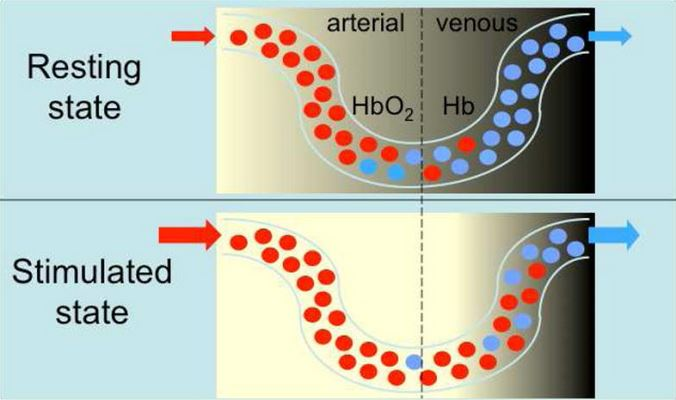
\includegraphics[width=.52\textwidth]{figures/aBackground/bold_response}  
	\caption{Illustration of how the difference in oxygen concentration in the hemoglobin change the magnetic properties, resulting in a measurable difference\cite{Glover2011}.}
	\label{fig:back:bold} 
\end{figure}


Strengths and weaknesses: All of the resolution mentioned above as well as being non-invasive. It can provide high resolution of anatomical structures and localization and visualization of vessels. Furthermore it can provide information of white matter connectivity through Diffusion Tensor Imaging. The downside is BOLD signals are were sensible to noise as the original signal is often lower than the noise. Additionally the loud scanner noise may distract patients during fMRI scans. 
\cite{Glover2011}

Major factors when doing fMRI:
The analysis of fMRI data is made complex by a number of factors. First, the data are liable to a number of artifacts, such as those caused by head movement. Second, there are a number of sources of variability in the data, including variability between individuals and variability across time within individuals. Third, the dimensionality of the data is very large, which causes a number of challenges in comparison to the small datasets that many scientists are accustomed to working with. The major components of fMRI analysis are meant to deal with each of these problems. \cite{Glover2011} 
